\documentclass[a4paper,12pt,twocolumn]{article}
\usepackage{geometry}
\geometry{margin=0.5in}
\usepackage[utf8]{inputenc}
\usepackage[most]{tcolorbox}
\usepackage{chemmacros}
\usepackage{graphicx}
\usepackage[version=4]{mhchem}
\usepackage{nopageno}
\usepackage{tikz}

\newtcolorbox{Box1}[2][]{
                lower separated=false,
                colback=white!80!gray,
colframe=white, fonttitle=\bfseries,
colbacktitle=white!50!gray,
coltitle=black,
enhanced,
attach boxed title to top left={xshift=0.5cm,yshift=-2mm},
title=#2,#1}


\newtcolorbox{Box2}[2][]{
                lower separated=false,
                colback=white,
colframe=black,fonttitle=\bfseries,
colbacktitle=black,
coltitle=white,
enhanced,
attach boxed title to top left={yshift=-0.1in,xshift=0.15in},
                 boxed title style={boxrule=0pt,colframe=white,},
title=#2,#1}

\newtcolorbox{Box3}[2][]{
                lower separated=false,
                colback=white!80!gray,
colframe=white!20!black,fonttitle=\bfseries,
colbacktitle=white!30!gray,
coltitle=black,
enhanced,
attach boxed title to top left={xshift=0.5cm,
        yshift=-2mm},
title=#2,#1}

\newtcolorbox{Box4}[2][]{arc=0mm,
                lower separated=false,
                colback=white!80!gray,
colframe=white!20!black,fonttitle=\bfseries,
colbacktitle=white!30!gray,
coltitle=black,
enhanced,
attach boxed title to top left={xshift=0.5cm,
        yshift=-2mm},
title=#2,#1}

\newcommand{\oxi}[2]{%
    \stackrel{#1}{\mathrm{#2}}
}%
\DeclareUnicodeCharacter{2212}{-}

\begin{document}

\begin{center}
\huge{Solution} \\[10pt]
\end{center}


\section{Solution}
\begin{itemize}
\item A \textbf{solution} is a homogeneous mixture of two or more substances in \textbf{microscopic level}. 
\item The \textbf{solute} is the substance present in a smaller amount, and the \textbf{solvent} is the substance present in a larger amount. 
\item A solution may be gaseous (such as air), solid (such as an alloy), or liquid (seawater, for example).
\end{itemize}

\section{Types of Solution}
\begin{itemize}
\item No restriction on the nature of the substances involved and  six types of solutions can be distinguished depending on the original states (solid, liquid, or gas) of the solution components:
\end{itemize}
\begin{table}[h]
\small
\centering
\def\arraystretch{1.2}
\begin{tabular}{|p{1.5cm}|p{1.5cm}|p{1.5cm}|p{2cm}|}
\hline Compo- \ nent \ 1 & Comp- \ onent \ 2 & State of \ Resulting Solution & Examples \\
\hline Gas & Gas & Gas & Air \\
\hline Gas & Liquid & Liquid &  Soda water \ ($\ce{CO2}$ in \ water ) \\
\hline Gas & Solid & Solid & $\ce{H2}$ gas in palladium \\
\hline Liquid & Liquid & Liquid & Ethanol in water \\
\hline Solid & Liquid & Liquid & $\mathrm{NaCl}$ in water \\
\hline Solid & Solid & Solid & \textbf{Brass:} \ (Cu/Zn) \ \textbf{solder:} \ (Sn/Pb)\\
\hline
\end{tabular}
\caption{Types of Solutions}
\end{table}

\section{Classification Based on the Capacity to Dissolve a Solute}
\begin{itemize}
\item A \textbf{saturated solution} contains the maximum amount of a solute that will dissolve in a given solvent at a specific temperature. 
\item An \textbf{unsaturated solution} contains less solute than it has the capacity to dissolve. 
\item A \textbf{supersaturated solution}, contains more solute than is present in a saturated solution. Supersaturated solutions are not very stable. In time, some of the solute will come out of a supersaturated solution as crystals.
\end{itemize}

\section{Crystallization from a Supersaturated Solution}

\begin{figure}[h]
\centering
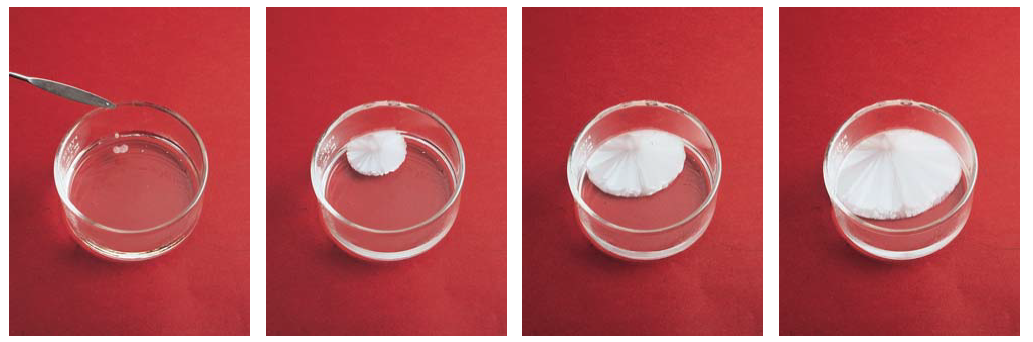
\includegraphics[width=0.4\textwidth]{Screenshot 2023-03-23 120914.png}
\caption{In a supersaturated sodium acetate solution (left), sodium acetate crystals rapidly form when a small seed crystal is added.}
\end{figure}


\begin{Box1}{}
\textbf{Crystallization is the process in which dissolved solute comes out of solution and forms crystals.}
\end{Box1}

\section{A Molecular View of the Solution Process}
\begin{itemize}
\item The intermolecular attractions that hold molecules together in liquids and solids also play a central role in the formation of solutions. 
\item When one substance (the solute) dissolves in another (the solvent), particles of the solute disperse throughout the solvent.
\item The solute particles occupy positions that are normally taken by solvent molecules. The ease with which a solute particle replaces a solvent molecule depends on the relative strengths of three types of interactions:
    \begin{enumerate}
        \item solvent-solvent interaction
        \item solute-solute interaction
        \item solvent-solute interaction
    \end{enumerate}
\end{itemize}

\begin{figure}[h]
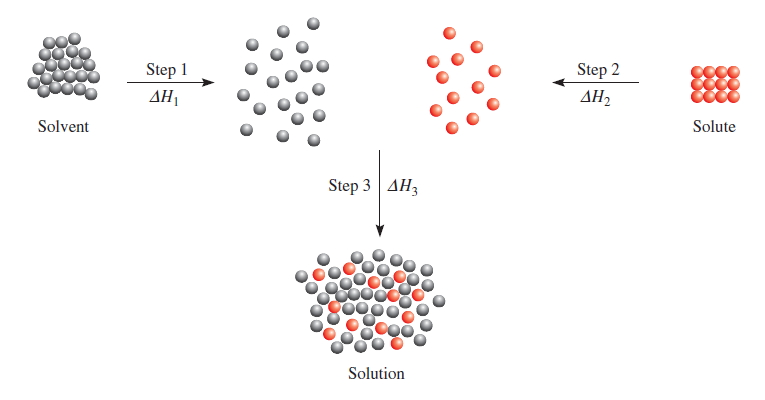
\includegraphics[width=0.5\textwidth]{Screenshot 2023-03-23 121400.png}
\caption{A molecular view of the solution process portrayed as taking place in three steps: First the solvent and solute molecules are separated (steps 1 and 2). Then the solvent and solute molecules mix (step 3).}
\end{figure}

\section{Exothermicity or Endo- \ thermicity}
\begin{itemize}
\item Step 1 is the separation of solvent molecules, and  Step 2 entails the separation of solute molecules. These steps require energy input to break attractive intermolecular forces; therefore, they are endothermic. 
\item In step 3 the solvent and solute molecules mix. This process can be exothermic or endothermic. 
\item The heat of solution $\ce{\Delta H_{soln}}$ is given by:
\begin{center}
$\ce{\Delta H_{soln} = \Delta H_{1} + \Delta H_{2} + \Delta H_{3}}$
\end{center}
\item If the solute-solvent attraction is stronger than the solvent-solvent attraction and solute-solute attraction, the solution process is favorable, or \textbf{exothermic ($\ce{\Delta H_{soln}}  < 0 $)}.
\item If the solute-solvent interaction is weaker than the solvent-solvent and solute-solute interactions, then the solution process is endothermic \textbf{($\ce{\Delta H_{soln}} > 0$)}.
\end{itemize}

\begin{Box2}{}
{\large Why a solute dissolves in a solvent at all if the attraction for its own molecules is stronger than the solute-solvent attraction?}
\end{Box2}
\begin{itemize}
\item The solution process is governed by two factors:
\begin{enumerate}
\item \textbf{One is energy, which determines whether a solution process is exothermic or endothermic.}
\item \textbf{The second factor is an inherent tendency toward disorder in all natural events.} When solute and solvent molecules mix to form a solution, there is an increase in randomness, or disorder. In the pure state, the solvent and solute possess a fair degree of order, characterized by the more or less regular arrangement of atoms, molecules, or ions in three-dimensional space. Much of this order is destroyed when the solute dissolves in the solvent. Therefore, the solution process is accompanied by an increase in disorder. 
\end{enumerate}
\item It is the increase in disorder of the system that favors the solubility of any substance, even if the solution process is endothermic.
\end{itemize}


\section{Solubility: Like Dissolves Like}
\begin{itemize}
\item \textbf{Solubility} is a measure of how much solute will dissolve in a solvent at a specific temperature. 
\item The saying \textbf{“like dissolves like”} is helpful in predicting the solubility of a substance in a given solvent. Two substances with intermolecular forces of similar type and magnitude are likely to be soluble in each other. 
\item For example, both carbon tetrachloride ($\ce{CCl4}$) and benzene ($\ce{C6H6}$) are nonpolar liquids. The only intermolecular forces present in these substances are dispersion forces. When these two liquids are mixed, they readily dissolve in each other, because the attraction between $\ce{CCl4}$ and $\ce{C6H6}$ molecules is comparable in magnitude to the forces between $\ce{CCl4}$ molecules and between $\ce{C6H6}$ molecules. 

\end{itemize}

\section{Concentration Units}
\begin{itemize}
\item The concentration of a solution is the amount of solute present in a given amount of solvent, or a given amount of solution.
\item Quantitative study of a solution requires knowing its concentration.
\end{itemize}

\section{Types of Concentration Units}
\begin{itemize}
\item \textbf{Percent By Mass:}\\
The percent by mass (also called percent by weight or weight percent) is the ratio of the mass of a solute to the mass of the solution, multiplied by 100 percent:\\
$\text { percent by mass } \\ =\dfrac{\text { mass of solute }}{\text { mass of solute }+ \text { mass of solvent }} \times 100 \%$

\begin{center}
$\text {or,  percent by mass}=\dfrac{\text { mass of solute}}{\text { mass of soln}} \times 100 \%$
\end{center}
The percent by mass is a unitless number because it is a ratio of two similar quantities.

\item \textbf{Mole Fraction(X):}\\ 
The mole fraction of a component
of a solution, say, component A, is written $X_A$ and is defined as:
\begin{center}
$X_{\mathrm{A}}=\dfrac{\text { moles of } \mathrm{A}}{\text { sum of moles of all components }}$
\end{center}

The mole fraction is also unitless, because it too is a ratio of two similar quantities.

\item \textbf{Molarity (M)}:\\ 
Molarity $(M)$, or molar concentration, which is the number of moles of solute per liter of solution. Molarity is defined as
$$
\text { molarity }=\dfrac{\text { moles of solute }}{\text { liters of solution }}
$$
This Equation can also be expressed algebraically as
$$
M=\dfrac{n}{V}
$$
where $n$ denotes the number of moles of solute and $V$ is the volume of the solution in liters.
Thus, the units of molarity are mol/L.
\item \textbf{Molality (m)}: \\
\textbf{Molality} is the number of moles of solute dissolved in 1 kg (1000g) of solvent - that is,
$$\text{molality } = \dfrac{\text {moles of solute}}{\text{mass of solvent (kg)}}$$
For example, to prepare a 1 molal, or 1m, sodium sulfate ($\ce{Na2SO4}$) aqueous solution, we need to dissovle 1 mole (142.0 g) of the substance in 1000 g (1 kg) of water. 
\end{itemize}

\section{Electrolytic Properties}
\begin{itemize}
\item All solutes that dissolve in water fit into one of two categories: \textbf{electrolytes} and \textbf{nonelectrolytes}. 
\item An electrolyte is a substance that, when dissolved in water, results in a solution that can conduct electricity. A nonelectrolyte does not conduct electricity when dissolved in water.

\end{itemize}

\begin{table}[h]
\centering
\begin{tabular}{|p{2cm}|l|l|}
\hline
Strong Electrolyte & Weak Electrolyte & Nonelectrolyte \\
\hline $\mathrm{HCl}$ & $\mathrm{CH}_3 \mathrm{COOH}$ & $\left(\mathrm{NH}_2\right)_2 \mathrm{CO}$ (urea) \\
$\mathrm{HNO}_3$ & $\mathrm{HF}$ & $\mathrm{CH}_3 \mathrm{OH}$ (methanol) \\
$\mathrm{HClO}_4$ & $\mathrm{HNO}_2$ & $\mathrm{C}_2 \mathrm{H}_5 \mathrm{OH}$ (ethanol) \\
$\mathrm{H}_2 \mathrm{SO}_4^*$ & $\mathrm{NH}_3$ & $\mathrm{C}_6 \mathrm{H}_{12} \mathrm{O}_6$ (glucose) \\
$\mathrm{NaOH}$ & $\mathrm{H}_2 \mathrm{O}^{\dagger}$ & $\mathrm{C}_{12} \mathrm{H}_{22} \mathrm{O}_{11}$ (sucrose) \\
$\mathrm{Ba}(\mathrm{OH})_2$ & & \\
Ionic & & \\
compounds & & \\ \hline
\end{tabular}
\caption{Classification of Solutes in Aqueous Soln.}
\end{table}

\section{Colligative Properties of Nonelectrolyte Solutions}
\begin{itemize}
\item Colligative properties (or collective properties) are properties that depend only on the number of solute particles in solution and not on the nature of the solute particles.
\item These properties are bound together by a common origin—they all depend on the number of solute particles present, regardless of whether they are atoms, ions, or molecules.
\end{itemize}

\section{Colligative Properties}
\begin{itemize}
\item The colligative properties are:
    \begin{enumerate}
        \item \textbf{vapor-pressure lowering}
        \item \textbf{boiling-point elevation}
        \item \textbf{freezing-point depression}, and
        \item \textbf{osmotic pressure}
    \end{enumerate}
\item Colligative properties of nonelectrolyte solutions - relatively dilute solutions, $\le 0.2 M$.
\end{itemize}

\section{Vapor-Pressure Lowering}
If a solute is \textbf{nonvolatile} (that is, it does not have a measurable vapor pressure), the vapor pressure of its solution is always less than that of the pure solvent. Thus, the relationship between solution vapor pressure and solvent vapor pressure depends on the concentration of the solute in the solution. This relationship is expressed by \textbf{Raoult's ${ }^{\dagger}$ law}, which states that the vapor pressure of a solvent over a solution, $P_1$, is given by the vapor pressure of the pure solvent, $P_1^{\circ}$, times the mole fraction of the solvent in the solution, $X_1$ :
$$
P_1=X_1 P_1^{\circ} \ldots (i)
$$
In a solution containing only one solute, $X_1=1-X_2$, where $X_2$ is the mole fraction of the solute. Equation (i) can therefore be rewritten as
or
$$
\begin{aligned}
P_1 &=\left(1-X_2\right) P_1^{\circ} \\
P_1 &=P_1^{\circ}-X_2 P_1^{\circ}
\end{aligned}
$$
so that
$$
P_1^{\circ}-P_1=\Delta P=X_2 P_1^{\circ}
$$
We see that the decrease in vapor pressure, $\Delta P$, is directly proportional to the solute concentration (measured in mole fraction).\\

\begin{Box2}{}
{\large Why is the vapor pressure of a solution less than that of the pure solvent?}
\end{Box2}
\begin{itemize}
\item One driving force in physical and chemical processes is an increase in disorder—the greater the disorder, the more favorable the process.
\item Vaporization increases the disorder of a system because molecules in a vapor have less order than those in a liquid. 
\item Because a solution is more disordered than a pure solvent, the difference in disorder between a solution and a vapor is less than that between a pure solvent and a vapor. Thus, solvent molecules have less of a tendency to leave a solution than to leave the pure solvent to become vapor, and the vapor pressure of a solution is less than that of the solvent.
\end{itemize}


\section{Boiling - Point Elevation}
\begin{itemize}
\item The boiling point of a solution is the temperature at which its vapor pressure equals the external atmospheric pressure.
\item Because the presence of a nonvolatile solute lowers the vapor pressure of a solution, it must also affect the boiling point of the solution. 


\begin{figure}[h]
\begin{center}
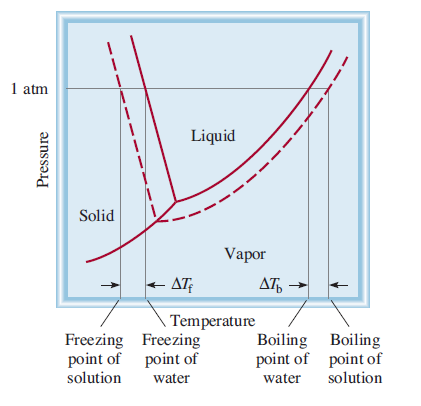
\includegraphics[width=0.5\textwidth, height=3.5in]{Screenshot 2023-03-23 161120.png}
\end{center}
\caption{Phase diagram illustrating the boiling-point elevation and freezing-point depression of aqueous solutions. The dashed curves pertain to the solution, and the solid curves to the pure solvent. The boiling point of the solution is higher than that of water, and the freezing point of the solution is lower than that of water.}
\end{figure}
\item The \textbf{boiling point elevation}\ $\left(\Delta T_b\right)$ is defined as the boiling point of the solution $\left(T_b\right)$ minus the boiling point of the pure solvent $\left(T_b^0\right)$ :
$$
\Delta T_{\mathrm{b}}=T_{\mathrm{b}}-T_{\mathrm{b}}^{\circ}
$$
Because $T_{\mathrm{b}}>T_{\mathrm{b}}^{\circ}, \Delta T_{\mathrm{b}}$ is a positive quantity.
The value of $\Delta T_{\mathrm{b}}$ is proportional to the vapor-pressure lowering, and so it is also proportional to the concentration (molality) of the solution. That is,
$$
\begin{gathered}
\Delta T_{\mathrm{b}} \propto m \\
\Delta T_{\mathrm{b}}=K_{\mathrm{b}} m
\end{gathered}
$$
where $m$ is the molality of the solution and $K_{\mathrm{b}}$ is the molal boiling-point elevation constant. The units of $K_{\mathrm{b}}$ are ${ }^{\circ} \mathrm{C} / \mathrm{m}$. It is important to understand the choice of concentration unit here. We are dealing with a system (the solution) whose temperature is not constant, so we cannot express the concentration units in molarity because molarity changes with temperature.
\end{itemize}

\begin{table}[h]
\centering
\def\arraystretch{1.5}
\begin{tabular}{|p{1.5cm}|p{1.4cm}|p{1.2cm}|p{1.4cm}|p{1.2cm}|}
\hline
Solvent &  Normal Freezing Point $({}^oC)^{*}$ & $K_f$ $({}^oC/m)$ & Normal Boiling Point $({}^oC)^{*}$ & $K_b$ $({}^oC/m)$\\
\hline Water & 0 & 1.86 & 100 & 0.52 \\ \hline
Benzene & 5.5 & 5.12 & 80.1 & 2.53 \\ \hline
Ethanol & -117.3 & 1.99 & 78.4 & 1.22 \\ \hline
Acetic acid & 16.6 & 3.90 & 117.9 & 2.93 \\ \hline
Cyclo hexane & 6.6 & 20.0 & 80.7 & 2.79\\ \hline
\end{tabular}
\caption{Molal Boiling-Point Elevation and Freezing-Point Depression Constants of Several Common Liquids. (*Measured at $1 \mathrm{~atm}$.)}
\end{table}


\section{Freezing - Point Depression}
\begin{itemize}
\item Freezing-point depression is the decrease of the freezing point of a solvent on the addition of a non-volatile solute. Examples include salt in water and alcohol in water.
\item It is defined as the freezing point of the pure solvent minus the freezing point of the solution.


\begin{figure}[h]
\begin{center}
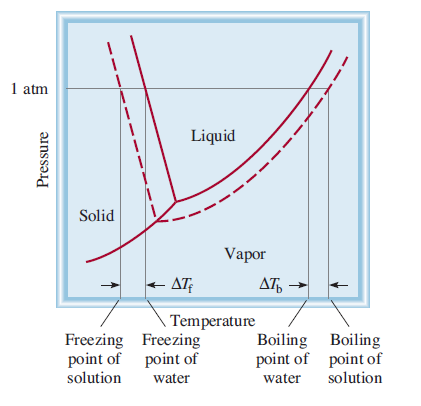
\includegraphics[width=0.26\textwidth, keepaspectratio]{Screenshot 2023-03-23 161120.png}
\end{center}
\end{figure}

\item The \textbf{freezing point depression} $\left(\Delta T_f\right)$ is defined as the freezing point of the pure solvent $\left(T_f^{\circ}\right)$ minus the freezing point of the solution $\left(T_f\right)$ :
$$
\Delta T_{\mathrm{f}}=T_{\mathrm{f}}^{\circ}-T_{\mathrm{f}}
$$
Because $T_{\mathrm{f}}^{\circ}>T_{\mathrm{f}}, \Delta T_{\mathrm{f}}$ is a positive quantity. Again, $\Delta T_{\mathrm{f}}$ is proportional to the concentration of the solution:
$$
\begin{gathered}
\Delta T_{\mathrm{f}} \propto m \\
\Delta T_{\mathrm{f}}=K_{\mathrm{f}} m
\end{gathered}
$$
where $m$ is the concentration of the solute in molality units, and $K_{\mathrm{f}}$ is the molal freezing-point depression constant (see Table 3). Like $K_{\mathrm{b}}, K_{\mathrm{f}}$ has the units ${ }^{\circ} \mathrm{C} / \mathrm{m}$.
\end{itemize}
\section{Qualitative Explanation of the Freezing-Point Depression}
\begin{itemize}
\item Freezing involves a transition from the disordered state to the ordered state. For this to happen, energy must be removed from the system. 
\item Because a solution has greater disorder than the solvent, more energy needs to be removed from it to create order than in the case of a pure solvent. 
\item Therefore, the solution has a lower freezing point than its solvent. Note that when a solution freezes, the solid that separates is the pure solvent component.
\end{itemize}

\section{Osmotic Pressure}
\begin{itemize}
\item Osmosis is the selective passage of solvent molecules through a semipermeable membrane from a dilute solution to a more concentrated one.
\item The osmotic pressure ($\pi$) of a solution is the pressure required to stop osmosis.
\end{itemize}
\begin{figure}[h]
\centering
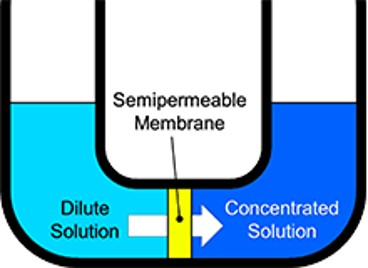
\includegraphics[width=0.185\textwidth, keepaspectratio]{reverse1.jpg} \qquad
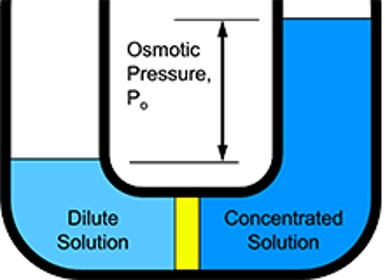
\includegraphics[width=0.185\textwidth, keepaspectratio]{reverse2.jpg}
\end{figure}
\begin{figure}[h]
\centering
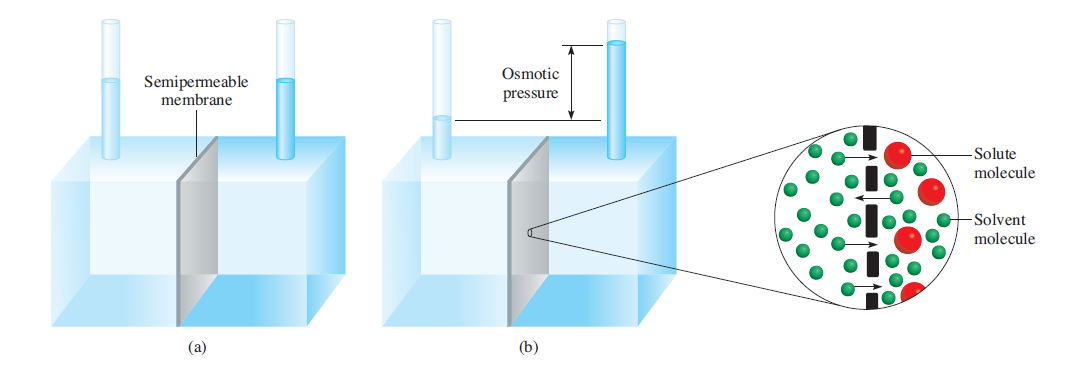
\includegraphics[width=0.5\textwidth]{Screenshot 2023-03-24 011415.png}
\caption{Osmotic pressure. (a) The levels of the pure solvent (left) and of the solution (right) are equal at the start. (b) During
osmosis, the level on the solution side rises as a result of the net fl ow of solvent from left to right. The osmotic pressure is equal to
the hydrostatic pressure exerted by the column of fluid in the right tube at equilibrium. Basically, the same effect occurs when the pure
solvent is replaced by a more dilute solution than that on the right.}
\end{figure}
\section{Driving Force for Osmosis}
\begin{itemize}
\item Because the vapor pressure of pure water is higher than the vapor pressure of the solution, there is a net transfer of water from the left beaker to the right one. 
\item A similar driving force causes water to move from the pure solvent into the solution during osmosis.
\end{itemize}
\begin{figure}[h]
\begin{center}
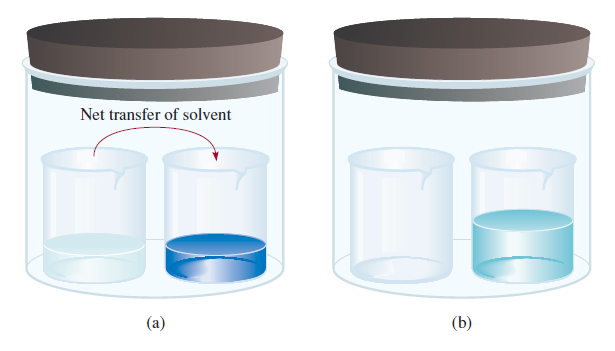
\includegraphics[width=0.4\textwidth]{Screenshot 2023-03-23 155651.png}
\end{center}
\caption{(a) Unequal vapor
pressures inside the container
lead to a net transfer of water
from the left beaker (which
contains pure water) to the right
one (which contains a solution).
(b) At equilibrium, all the water
in the left beaker has been
transferred to the right beaker.
This driving force for solvent
transfer is analogous to the
osmotic phenomenon that is
shown}
\end{figure}
The osmotic pressure of a solution is given by:
\begin{center}
$\mathrm{\pi = MRT}$
\end{center}
where \textbf{M} is the molarity of solution, \textbf{R} is the gas constant ($\mathrm{0.0821 \quad L . atm/K . mol}$), and
T is the absolute temperature. The osmotic pressure, $\pi$, is expressed in atm. Because
osmotic pressure measurements are carried out at constant temperature, we express the
concentration in terms of the more convenient units of molarity rather than molality.\\
\section{Classification of Solution Based on Osmotic Pressure}
\begin{itemize}
\item If two solutions are of equal concentration and, hence, have the same osmotic pressure, they are said to be \textbf{isotonic}. 
\item If two solutions are of unequal osmotic pressures, the more concentrated solution is said to be \textbf{hypertonic} and the more dilute solution is described as \text{hypotonic}.

\end{itemize}
\section{Reverse Osmosis}
\begin{itemize}
\item If pressure greater than the osmotic pressure is applied to the high concentration the direction of water flow through the membrane can be reversed. This is called reverse osmosis. 
\begin{figure}[h]
\centering
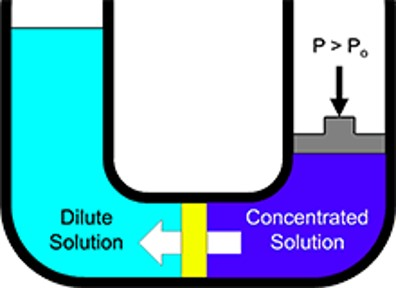
\includegraphics[width=0.25\textwidth, keepaspectratio]{reverse3.jpg}
\end{figure}

\end{itemize}
\section{Desalination of Water}
\begin{enumerate}
\item Distillation
\item Freezing
\item Reverse Osmosis
\end{enumerate}
\section{Reverse Osmosis for Desalination of Seawater}
\begin{itemize}
\item Reverse osmosis uses high pressure to force water from a more concentrated solution to a less concentrated one through a semipermeable membrane. 
\item The osmotic pressure of seawater is about 30 atm—this is the pressure that must be applied to the saline solution in order to stop the flow of water from left to right. If the pressure on the salt solution were increased beyond 30 atm, the osmotic flow would be reversed, and freshwater would actually pass from the solution through the membrane into the left compartment. 

\end{itemize}
\section{Advantage and Disadvantage}
\begin{itemize}
\item Desalination by reverse osmosis is considerably cheaper than distillation and it avoids the technical difficulties associated with freezing. 
\item The main obstacle to this method is the development of a membrane  that is permeable to water but not to other dissolved substances and that can be used on a large scale for prolonged periods under high-pressure conditions. Once this problem has been solved, and present signs are encouraging, reverse osmosis could become a major desalination technique.
\end{itemize}
\end{document}